%----------------------------------------------------------------------------------------
%	PACKAGES AND DOCUMENT CONFIGURATIONS
%----------------------------------------------------------------------------------------
\documentclass[article, a4paper, 12pt, oneside]{memoir}

% Margins
\usepackage[top=3cm,left=2cm,right=2cm,bottom=3cm]{geometry}

% Encondings
\usepackage[utf8]{inputenc}

% Language
\usepackage[portuguese]{babel}

% Graphics and images
\usepackage{graphicx}
	\graphicspath{{../images/}}

% Listings
\usepackage{listings}

% Color
\usepackage[dvipsnames]{xcolor}

% Tables
\usepackage{tabularx}

% Math symbols
\usepackage{amssymb}

% Paragraph Spacing
\usepackage{parskip}
\usepackage{indentfirst}
\setlength{\parskip}{0.5cm}

% Hyperreferences
\usepackage{hyperref}

% Repeated commands
\usepackage{expl3}
\ExplSyntaxOn
\cs_new_eq:NN \Repeat \prg_replicate:nn
\ExplSyntaxOff

% Header and Footer Things
\usepackage{wallpaper}
\usepackage{fancyhdr}

% Following code to edit the pagestyle
\pagestyle{fancy}
\fancyhf{}
\rhead{Meat Wagons}
\lhead{\leftmark}
\rfoot{Página \thepage}

% Commands
\usepackage{xargs}

%% Linked Email
\newcommand{\email}[1]{
{\texttt{\href{mailto:#1}{#1}} }
}

%----------------------------------------------------------------------------------------
%	DOCUMENT INFORMATION
%----------------------------------------------------------------------------------------
% Title
\title{\Huge \texttt{Meat Wagons - Transporte de Prisioneiros} }
% Authors
\author{
\LARGE \textbf{Turma 2 Grupo 3}\\\\
\begin{tabular}{l r}
	\email{up201806250@fe.up.pt} & Diogo Samuel Gonçalves Fernandes	\\
	\email{up201806490@fe.up.pt} & Hugo Miguel Monteiro Guimarães \\
	\email{up201806554@fe.up.pt} & Telmo Alexandre Espirito Santo Baptista	\\
\end{tabular}
}

%\institute{Faculdade de Engenharia da Universidade do Porto \\ Bases de Dados (BDAD) - Turma 4, grupo 6}

% Date for the report
\date{\today}

% Table of Contents
\addto\captionsportuguese{\renewcommand*\contentsname{Índice}}

%----------------------------------------------------------------------------------------
%	DOCUMENT
%----------------------------------------------------------------------------------------
\begin{document}
%----------------------------------------------------------------------------------------
%	Front Page
%----------------------------------------------------------------------------------------
% Title Author and Date
\maketitle

% More information for front page
\begin{center}
\textbf{Projeto CAL - 2019/20 - MIEIC}
\Repeat{2}{\linebreak}
\begin{tabular}{l r}
	\textbf{Professor das Aulas Práticas}: & \href{https://sigarra.up.pt/feup/pt/func_geral.formview?p_codigo=419241}{Rosaldo José Fernandes Rossetti}
\end{tabular}
\Repeat{4}{\linebreak}
% FEUP Logo

\includegraphics[scale=0.4]{FEUP-logo.jpg}

\end{center}

\newpage
% Header Image
\CenterWallPaper{0.1}{FEUP-logo.jpg}
\addtolength{\wpXoffset}{-7.5cm}
\addtolength{\wpYoffset}{13.8cm}

%----------------------------------------------------------------------------------------
%	TABLE OF CONTENTS
%----------------------------------------------------------------------------------------
\tableofcontents*

\newpage
%----------------------------------------------------------------------------------------
%	CHAPTER 1 - Descrição do Problema
%----------------------------------------------------------------------------------------
\chapter[Descrição do Problema][Descrição do Problema]{Descrição do Problema} \label{\thechapter}

Os transportes de prisioneiros entre diversos estabelecimentos como, por exemplo, as prisões, esquadras e tribunais são feitos utilizando veículos que se encontrem adaptados ao serviço. Estes veículos têm a necessidade de serem altamente resistentes, uma vez que é necessário garantir que os prisioneiros não conseguem escapar.

Para este projeto, queremos otimizar o percurso dos veículos de forma a recolher e entregar os prisioneiros nos pontos de interesse. De modo a cumprir o pretendido, é possível dividir o nosso projeto nas seguintes fases:

\subsection{Primeira Iteração - Recolha de prisioneiros utilizando um único veículo}
	Inicialmente, consideramos que só existe um único veículo para realizar todos os serviços.
	Com a primeira iteração pretende-se que apenas um veículo recolha os prisioneiros numa dada localização.
	É necessário ter em consideração obras nas vias públicas, uma vez que estas podem tornar certas zonas inacessíveis, inviabilizando o transporte de prisioneiros.

	É importante notar que a recolha só pode ser efetuada caso existam caminhos que liguem todos os pontos de interesse, ou seja, o grafo necessita de ser conexo.

\subsection{Segunda Iteração - Recolha de prisioneiros utilizando vários veículos}
	Durante a segunda iteração ter-se-à em consideração o diverso número de veículos que a frota possui. Os veículos vão diferir uns dos outros conforme um determinado tipo. Nesta fase do projeto irão existir veículos específicos para transportar tipos específicos de prisioneiros.

\subsection{Terceira Iteração - Recolha seletiva de prisioneiros utilizando um único veículo}
	Na terceira iteração será considerada a possibilidade de um veículo atender a diferentes pedidos de transporte de prisioneiros, com diversos pontos de interesse diferentes, desde que não afete consideravelmente o tempo de espera do pedido anterior e não ultrapasse a capacidade do veículo.
	
\subsection{Quarta Iteração - Recolha seletiva de prisioneiros utilizando vários veículos}
	A quarta iteração assemelha-se à terceira iteração, mas considerando um número variável de veículos disponíveis, tentando otimizar também o número de veículos utilizados.

\newpage

%----------------------------------------------------------------------------------------
%	CHAPTER 2 - Formalização do Problema
%----------------------------------------------------------------------------------------
\chapter[Formalização do Problema][Formalização do Problema]{Formalização do Problema} \label{\thechapter}

\section{Dados de Entrada}

$C_i$ - sequência de veículos, sendo $C_i(i)$ o seu i-ésimo elemento. Cada veículo é caraterizado por:
\begin{itemize}
	\item $capacity$ - número de prisioneiros que pode transportar
	\item $type$ - tipo de veículo
\end{itemize}

$R_i$ - sequência de pedidos de transporte de prisioneiros, sendo $R_i(i)$ o seu i-ésimo elemento. Cada pedido é caraterizado por:
\begin{itemize}
	\item $pickup$ - local de recolha dos prisioneiros
	\item $dest$ - local de destino dos prisioneiros
	\item $numPris$ - número de prisioneiros a serem transportados
	\item $type$ - tipo de prisioneiros
	\item $p_d$ - peso da distância no trajeto a efetuar
	\item $p_t$ - peso do tempo no trajeto a efetuar
\end{itemize}

$G_i = (V_i, E_i)$ - grafo dirigido pesado, composto por:
\begin{itemize}
	\item $V$ - vértices, representando pontos da rede viária, com:
		\begin{itemize}
			\item $ID$ - Identificador único do vértice
			\item $D$ - Densidade populacional no vértice
			\item $Adj \subseteq E$ - arestas que saiem do vértice
			\item $avg-speed$ - velocidade média na área em volta do vértice
			\item $reachable$ - se o vértice é alcançável a partir da central
		\end{itemize}
	\item $E$ - arestas, representando conexão entre dois pontos da rede viária, com:
		\begin{itemize}
			\item $ID$ - Identificador único da aresta
			\item $W_d$ - peso da aresta em relação à distância (representa a distância entre os dois vértices)
			\item $W_t$ - peso da aresta em relação ao tempo (representa o tempo médio que demora a percorrer a distância entre os dois vértices, considerando o tráfego normal naquela conexão da rede viária)
			\item $open$ - se a conexão entre os vértices está aberta, isto é, se a rua estiver cortada por alguma razão então não é possível utilizar esta conexão
		\end{itemize}
\end{itemize}

$S$ - vértice da central

\section{Dados de Saída}

$G_f = (V_f, E_f)$ - grafo dirigido pesado, tendo $V_f$ e $E_f$ os mesmos atributos que $V_i$ e $E_i$, excluindo atributos específicos do algoritmo utilizado

$C_f$ - sequência de veículos com os serviços a realizar, sendo $C_f(i)$ o seu i-ésimo elemento. Cada veículo é caraterizado por:
\begin{itemize}
	\item $S$ - sequência de serviços a realizar, sendo $S(i)$ o seu i-ésimo elemento. Cada serviço é caraterizado por:
	\begin{itemize}
		\item $emptySeats$ - número de lugares vazios
		\item $R_f$ - sequência de pedidos atendidos, sendo $R_f(i)$ o seu i-ésimo elemento. Cada pedido atendido é caraterizado por:
		\begin{itemize}
			\item $pickupHour$ - hora de chegada ao local de recolha
			\item $destHour$ - hora de chegada ao local de destino
			\item $p_d$ - peso da distância no trajeto a efetuar
			\item $p_t$ - peso do tempo no trajeto a efetuar
		\end{itemize}
		\item $P = { e ~ \in ~ E_i }$ - sequência de arestas a percorrer, sendo $P(i)$ o seu i-ésimo elemento
		\item $dist$ - distância percorrida no serviço
		\item $startHour$ - hora esperada de ínicio do serviço
		\item $endHour$ - hora esperada de termino do serviço
	\end{itemize}
\end{itemize}

\newpage
\section{Restrições}

\subsection{Sobre os dados de entrada}

\begin{itemize}
	\item $\forall i ~ \in ~ [0, \vert C_i \vert [: capacity(C_i(i)) > 0$, uma vez que não faz sentido os veículos não poderem transportar prisioneiros
	\item $\forall r ~ \in ~ R_i, dest(r)$ deve pertencer ao mesmo componente fortemente conexo do grafo $G_i$ que o vértice $S$, uma vez que o veículo tem de ser capaz de voltar à central
	\item $\forall r ~ \in ~ R_i, numPris(r) > 0$, uma vez que não faz sentido ter um pedido para transportar zero prisioneiros
	\item $\forall r ~ \in ~ R_i, p_d \geq 0 \wedge p_t \geq 0 \wedge (p_d \neq 0 \vee p_t \neq 0)$
	\item $\forall v ~ \in ~ V_i, avg$-$speed(v) > 0$
	\item $\forall e ~ \in ~ E_i, W_d(e) > 0 \wedge W_t(e) > 0$, uma vez que o peso da aresta representa a distância ou o tempo médio necessário para percorrer a aresta, se esta distância ou tempo forem zero estaremos num ciclo no mesmo vértice
	\item $\forall e ~ \in ~ E_i, e$ deve ser uma rua ao qual os veículos possam utilizar, ruas que os veículos não tenham permissão para entrar não são incluídas no grafo $G_i$
	\item $S ~ \in ~ V_i$, uma vez que a central é um vértice do grafo $G_i$
\end{itemize}

\subsection{Sobre os dados de saída}

\begin{itemize}
	\item $\vert C_f \vert \leq \vert C_i \vert $ - não se pode usar mais veículos que os disponíveis
	\item $\forall v_f ~ \in ~ V_f, \exists v_i ~ \in ~ V_i$ tal que $v_i$ e $v_f$ têm os mesmos valores para todos os atributos, com exceção de atributos específicos aos algoritmos utilizados
	\item $\forall e_f ~ \in ~ E_f, \exists e_i ~ \in ~ E_i$ tal que $e_i$ e $e_f$ têm os mesmo valores para todos os atributos, com exceção de atributos específicos aos algoritmos utilizados
	\item $\forall r_f ~ \in ~ R_f, \exists r_i ~ \in ~ R_i$ tal que $r_f$ e $r_i$ têm os mesmo valores para os atributos $p_d$ e $p_t$
	\item $\forall c ~ \in ~ C_f, \forall s ~ \in ~ S(c), 0 \leq emptySeats < capacity(c)$ pois cada serviço deve ter pelo menos um prisioneiro, e não pode haver sobrelotação do veículo
	\item $\forall c ~ \in ~ C_f, \forall s ~ \in ~ S(c), \vert R_f(s) \vert > 0$ uma vez que só faz sentido realizar um serviço se existir mais de um pedido de transporte de prisioneiros
	\item $\forall c ~ \in ~ C_f, \forall s ~ \in ~ S(c), endHour(s) > startHour(s)$
	\item $\forall c ~ \in ~ C_f, \forall s ~ \in ~ S(c), startHour(s) < pickupHour(\forall r ~ \in ~ R_f) < endHour(s) ~ \wedge ~ startHour(s) < destHour(\forall r ~ \in ~ R_f) \leq endHour(s)$
	\item $\forall c ~ \in ~ C_f, \forall s ~ \in ~ S(c), \forall r ~ \in ~ R_f(s), index(dest(r)) > index(pickup(r))$
\end{itemize}

\section{Função objetivo}

A solução ótima passa por minimizar a soma ponderada da distância percorrida e o tempo do serviço de um determinado veículo, que resulta na seguinte função:

$\sum_{c ~ \in ~ C_f} \sum_{s ~ \in ~ S} \sum_{e ~ \in ~ P} (W_d(e) * max(p_d(R_f(s))) + W_t(e) * max(p_t(R_f(s))$

\begin{itemize}
	\item $max(p_d(R_f(s))$ - é o maior valor para o peso da distância numa determinada sequência de pedidos de um serviço de um veículo
	\item $max(p_t(R_f(s))$ - é o maior valor para o peso do tempo numa determinada sequência de pedidos de um serviço de um veículo
\end{itemize}

Deste modo, obtivemos a função objetivo para o nosso problema que se encontra acima.

\newpage
%----------------------------------------------------------------------------------------
%	CHAPTER 3 - Perspectiva de solução
%----------------------------------------------------------------------------------------
\chapter[Perspectiva de solução][Perspectiva de solução]{Perspectiva de solução} \label{\thechapter}

\section{Pré-processamento dos dados de entrada}

\subsection{Grafo}
Partindo da central, todos os vértices que não forem alcançáveis têm a variável $reachable$ definida como falsa.

Além disso, todas os vértices do grafo que não pertençam à componente fortemente conexa de origem devem ser marcados como inacessíveis ($reachable$ é colocado a falso).

\subsection{Pedidos de transporte de prisioneiros}
Remover todos os pedidos de transporte de prisioneiros que não pertençam ao grafo pré-processado, isto é, remover aqueles que façam parte de vértices que têm a componente $reachable$ definida como falsa.

Também devemos organizar os pedidos de transporte de prisioneiros por ordem decrescente do número de prisioneiros a transportar, facilitando, em seguida, o alocamento de veículos para o seu transporte.

\subsection{Veículos para transporte de prisioneiros}
Relativamente ao pré-processamento dos veículos de transporte, devemos organizá-los por ordem decrescente de capacidade. Deste modo, como também temos os pedidos de transporte de prisioneiros organizados por ordem decrescente do número de prisioneiros a transportar podemos potencialmente minizar o número de veículos utilizados.

\section{Identificação do problema}

A empresa de transporte de prisioneiros Meat Wagons necessita de transportar os prisioneiros  de um ponto de recolha até um determinado destino. De modo a otimizar este transporte, a empresa optou por procurar o caminho mais eficiente para a efetuar a viagem.

Na primeira iteração, onde apenas está disponível um veículo, que realiza os pedidos de transporte um de cada vez, este problema trata-se do \textbf{caminho mais curto} entre a origem e o local de recolha seguido do \textbf{caminho mais curto} entre o local de recolha e o destino. A segunda iteração é semelhante à primeira iteração, variando apenas o número de veículos disponíveis para realizar os pedidos.

Na terceira iteração, um veículo poderá realizar vários pedidos simultâneamente, equiparando-se assim ao \textbf{Travelling Salesman Problem}, com restrições no vértice de origem, e na ordem de visita dos vértices.

Na quarta e última iteração, não só varia o número de veículos disponíveis, como também o número de pedidos de transporte que um veículo pode realizar num único serviço, equiparando-se ao problema designado por \textbf{Vehicle Routing Problem}, uma generalização do \textbf{Travelling Salesman Problem}, um problema \emph{NP-díficil}.

Vale também realçar que os veículos devem retornar para a central no fim do serviço.

\section{Caminho mais curto}
Este é o problema referido na primeira e segunda iteração, e trata-se de encontrar o percurso mais curto e eficiente entre dois pontos, ou entre todos os pares de pontos do grafo.

\subsection{Entre dois pontos}
Entre os vários algoritmos que existem para calcular o caminho mais curto entre dois pontos destacam-se os seguintes algoritmos:

\subsubsection{Algoritmo de Dijkstra}
Este algoritmo foi concebido por \href{https://en.wikipedia.org/wiki/Edsger_W._Dijkstra}{Edsger W. Dijkstra} e resolve problemas do caminho mais curto de uma única origem em grafos que possuam pesos não negativos.

Para poder aplicar este algoritmo é necessário que cada vértice guarde a seguinte informação:
\begin{itemize}
	\item $W$ - custo mínimo até ao local da origem (combinação linear da distância e tempo, como visto na função objetivo)
	\item $path$ - vértice antecessor no caminho mais curto
\end{itemize}

O algoritmo de Dijkstra pode utilizar uma $priority$ $queue$ ou um $array$ para inserir os novos vértices.
Este consiste em inicializar os vértices, o que se pode fazer em tempo linear $O(|V|)$. Seguidamente, inicializar a estrutura auxiliar, que neste caso consideramos a $priority queue$ devido a ter maior eficiência relativamente ao $array$, com o vértice origem.

Processam os vértices que se encontram na $queue$ extraindo-os e seguidamente percorrendo cada aresta do vértice a ser processado. Posteriormente, se o custo relativo ao vértice de destino da aresta for maior do que o custo do caminho atual, terá que se atualizar o vértice de destino e inserindo na $priority$ $queue$ caso ele ainda não esteja na fila de processamento ou fazendo a operação $DECREASE-KEY$ caso este já esteja na fila de processamento.

As operações de inserção, extração e $DECREASE-KEY$ têm complexidade temporal $O(log(N))$. Dado que é necessário percorrer todos os vértices e arestas resulta numa complexidade de $O((|V| + |E|)*log(|V|))$.

Assim podemos concluir que o tempo de execução do algoritmo é $O((|V| + |E|)*log(|V|))$.

\newpage
O pseudo-código para implementar este algoritmo é o seguinte:

\begin{lstlisting}[frame=single, mathescape=true]
FOR EACH v $\in$ V DO
  COST(v) $\leftarrow$ $\infty$
  PATH(v) $\leftarrow$ NULL

COST(s) $\leftarrow$ 0
Q $\leftarrow$ $\varnothing$ // MIN PRIORITY QUEUE
INSERT(Q, (s, COST(s)))
WHILE Q $\neq$ $\varnothing$ DO
  v $\leftarrow$ EXTRACT-MIN(Q)
  FOR EACH w $\in$ Adj(v) DO
    IF COST(w) > COST(v) + WEIGHT(v, w) THEN
      COST(w) $\leftarrow$ COST(v) + WEIGHT(v, w)
      PATH(w) $\leftarrow$ v
      IF w $\notin$ Q THEN
        INSERT(Q, (w, COST(w)))
      ELSE
        DECREASE-KEY(Q, (w, COST(w)))
\end{lstlisting}

Este algoritmo destaca-se pela sua facilidade de implementação, porém o algoritmo pode explorar demasiados vértices desnecessários.

A ineficiência do algoritmo pode ser visto na imagem abaixo:

\begin{figure}[h]
\centering
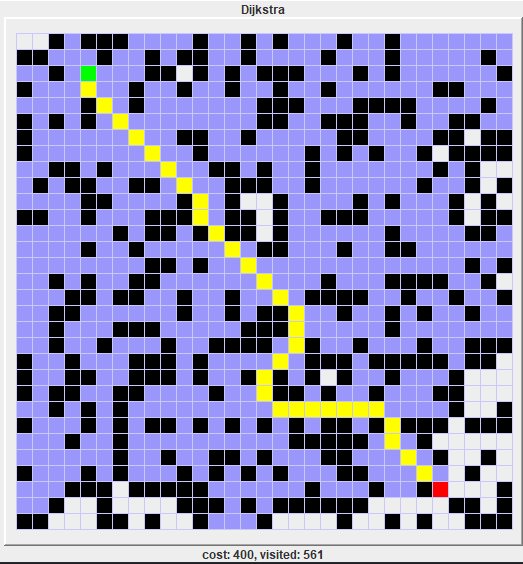
\includegraphics[scale=0.4]{dijkstra}
\caption{\emph{Dijkstra's algorithm}}
\begin{tabular}{ l r }
\color{black} $\blacksquare$ \color{black} walls & \color{Periwinkle} $\blacksquare$ \color{black} visited \\
\color{green} $\blacksquare$ \color{black} origin & \color{red} $\blacksquare$ \color{black} destination \\
\color{yellow} $\blacksquare$ \color{black} shortest path
\end{tabular}
\end{figure}

\subsubsection{Algoritmo de Bellman-Ford}
O algoritmo de Bellman-Ford corresponde a uma extensão do algoritmo de Dijkstra permitindo a existência de pesos negativos nas arestas, sendo mais lento que o de Dijkstra por esse mesmo motivo.

Uma vez que foi imposta a restrição de pesos não negativos nas arestas, este algoritmo não se vê útil, uma vez que não se vê necessário tratar pesos negativos.

\subsubsection{Algoritmo A*}
O algoritmo A*, desenvolvido por \href{https://en.wikipedia.org/wiki/Peter_E._Hart}{Peter Hart}, \href{https://en.wikipedia.org/wiki/Nils_John_Nilsson}{Nils Nilsson} e \href{https://en.wikipedia.org/wiki/Bertram_Raphael}{Bertram Raphael}, pode ser visto como uma extensão do algoritmo de Dijkstra, usando heurística para guiar a sua pesquisa.

Em cada iteração, o algoritmo precisa decidir qual caminho processar, baseando-se no custo  do caminho desde a origem até ao ponto atual e numa estimativa do custo do caminho desde o vértice adjacente a testar até ao destino, isto é o algoritmo visa minimizar a seguinte função
\begin{equation}
f(n) = g(n) + h(n)
\end{equation}
onde $n$ é o próximo vértice do caminho, $g(n)$ o custo desde a origem até $n$ e $h(n)$ uma estimativa do custo mínimo desde $n$ até ao destino.

Uma possível implementação do algoritmo está demonstrada no seguinte pseudo-código:
\begin{lstlisting}[frame=single, mathescape=true]
RECONSTRUCT_PATH(current)
  path $\leftarrow$ {current}
  WHILE PATH(current) $\neq$ NULL
    current $\leftarrow$ PATH(current)
    PREPEND(path, current)
  RETURN path

A_STAR(start, goal, heuristic)
  FOR EACH v $\in$ V DO
    G_COST(v) $\leftarrow$ $\infty$
    F_COST(v) $\leftarrow$ $\infty$
    PATH(v) $\leftarrow$ NULL

  G_COST(start) $\leftarrow$ 0
  F_COST(start) $\leftarrow$ heuristic(start) // G_COST(start)+heuristic(start)
  Q $\leftarrow$ $\varnothing$ // MIN PRIORITY QUEUE
  INSERT(Q, (start, F_COST(start)))
  WHILE Q $\neq$ $\varnothing$ DO
    v $\leftarrow$ EXTRACT-MIN(Q)
    IF V = GOAL
      RETURN RECONSTRUCT_PATH(v)

    FOR EACH w $\in$ Adj(v) DO
      IF G_COST(w) > G_COST(V) + WEIGHT(v, w) THEN
        G_COST(w) $\leftarrow$ G_COST(v) + WEIGHT(v, w)
        PATH(w) $\leftarrow$ v
        F_COST(w) $\leftarrow$ G_COST(w) + heuristic(w)
        IF w $\notin$ Q THEN
          INSERT(Q, (w, F_COST(w)))
        ELSE
          DECREASE-KEY(Q, (w, F_COST(w)))
\end{lstlisting}

O algoritmo A* é um algoritmo de elevada eficiência e otimização, sendo usado em muitos contextos, como nos sistemas de \href{https://en.wikipedia.org/wiki/Journey_planner}{encaminhamento de viagens} que corresponde às duas primeiras iterações do nosso problema.

A eficiência deste algoritmo pode ser observada comparando o número de vértices explorados durante a pesquisa com o algoritmo de Dijkstra, como é demonstrado na imagem abaixo:

\begin{figure}[h]
\centering
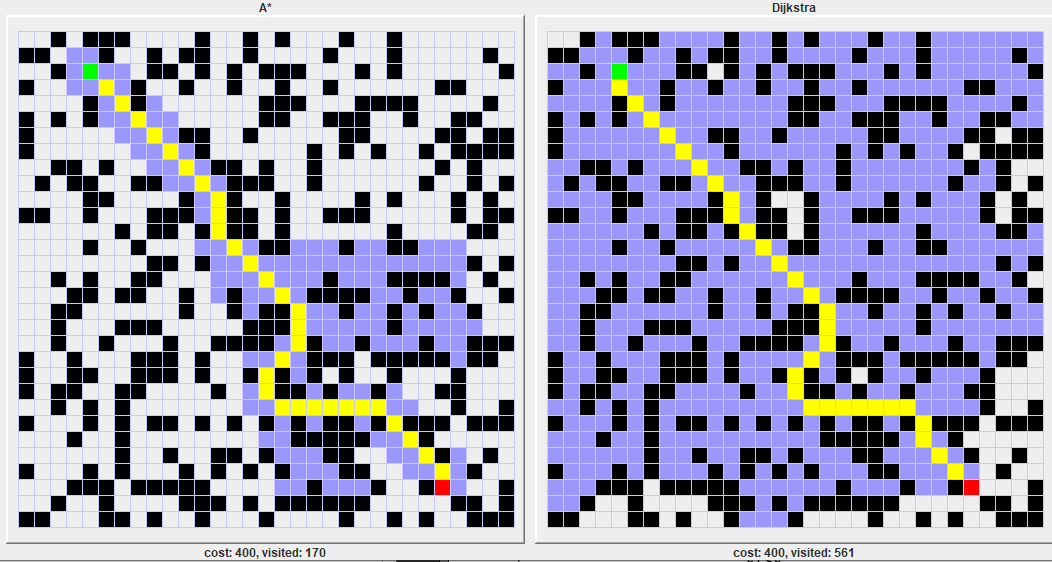
\includegraphics[scale=0.4]{pathfinder}
\caption{\emph{A* algorithm \textbf{vs.} Dijkstra's algorithm}}
\begin{tabular}{ l r }
\color{black} $\blacksquare$ \color{black} walls & \color{Periwinkle} $\blacksquare$ \color{black} visited \\
\color{green} $\blacksquare$ \color{black} origin & \color{red} $\blacksquare$ \color{black} destination \\
\color{yellow} $\blacksquare$ \color{black} shortest path
\end{tabular}
\end{figure}

\newpage
Embora a eficiência do algoritmo seja maior, o algoritmo A* não garante a solução ótima para todos os casos, ao contrário de algoritmos como o de Dijkstra. Esta desvantagem pode ser observada na imagem abaixo:

\begin{figure}[h]
\centering
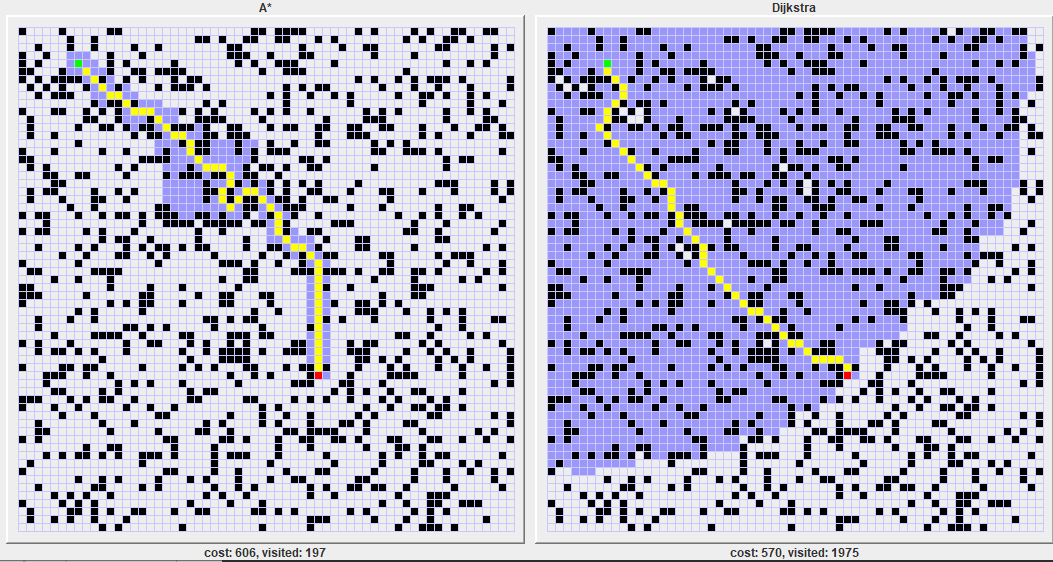
\includegraphics[scale=0.4]{pathfinder2}
\caption{\emph{A* algorithm \textbf{vs.} Dijkstra's algorithm}}
\begin{tabular}{ l r }
\color{black} $\blacksquare$ \color{black} walls & \color{Periwinkle} $\blacksquare$ \color{black} visited \\
\color{green} $\blacksquare$ \color{black} origin & \color{red} $\blacksquare$ \color{black} destination \\
\color{yellow} $\blacksquare$ \color{black} shortest path
\end{tabular}
\end{figure}

Analisando os resultados obtidos, é possível constatar que o algoritmo de Dijkstra visitou aproximadamente dez vezes mais vértices que o algoritmo A* ($1975 ~ \textbf{vs.} ~ 197$). Porém, o caminho mais curto encontrado pelo algoritmo A* não corresponde ao caminho com menor custo, uma vez que o caminho encontrado pelo algoritmo de Dijkstra possui um custo menor que o algoritmo de A* ($570 ~ \textbf{vs.} ~ 606$).

\subsection{Entre todos os pares de vértices}
É possível calcular o caminho entre todos os pares de vértices através de algoritmos, como a aplicação repetida do algoritmo de Dijkstra ou a utilização do algoritmo de Floyd-Warshall.

Estes algoritmos são bastante utilizados para pré-processamento de mapas de estradas, porém no nosso problema, como os pesos para a distância e o para o tempo variam de pedido para pedido, o pré-processamento dos caminhos mais curtos para todos os pares de vértices não traria nenhuma vantagem, apenas uma diminuição na eficiência do programa.

\newpage
\section{Caminho mais curto com vários pedidos}
Dada a possibilidade de um veículo realizar vários pedidos num único serviço, existirá um conjunto de locais de recolha e locais de destino a serem percorridos.

Deparámo-nos então com um problema similar ao \textbf{Travelling Salesman Problem}, um problema NP-difícil. Como se trata de um grafo dirigido é a versão assimétrica do problema \textbf{Travelling Salesman Problem}.

As soluções deste problema podem dividir-se em duas categorias:
\begin{itemize}
	\item \textbf{Soluções Exatas} - algoritmos que encontram a solução exata do problema
	\item \textbf{Soluções Aproximadas} - algoritmos que aproximam a solução do problema através de heurísticas e aproximações
\end{itemize}

\subsection{Soluções Exatas}
\subsubsection{Brute-force}
O método brute-force testa todas as permutações possíveis para o percurso, atualizando o caminho ótimo sempre que encontra um custo menor ao atual, resultando assim numa complexidade $O(n!)$, sendo $n$ o número de vértices a percorrer.

\subsubsection{Held-Karp}
O algoritmo de Held-Karp é um algoritmo de programação dinâmica que tem como objetivo resolver o \textbf{Travelling Salesman Problem}, utilizando formulas recursivas para dividir o problema.

O algoritmo apresenta uma complexidade temporal elevada, $O(2^nn^2)$, requirindo, assim, muito poder computacional para obter a solução ótima.

Embora este algoritmo obtenha a solução ótima para o problema, a sua implementação, dada as restrições impostas, pode ser muito complexa, pelo que serão priorizados os algoritmos de soluções aproximadas do problema, dado à sua simplicidade e flexibilidade.

\newpage
Analisando as complexidades dos algoritmos apresentados podemos verificar que o método de brute-force é mais eficiente para valores de $n$ menores que sete, sendo o algoritmo de Held-Karp mais eficiente para os restantes valores de $n$, sendo $n$ o número de vértices a percorrer, assim como se pode observar no gráfico seguinte:

\begin{figure}[h]
\centering
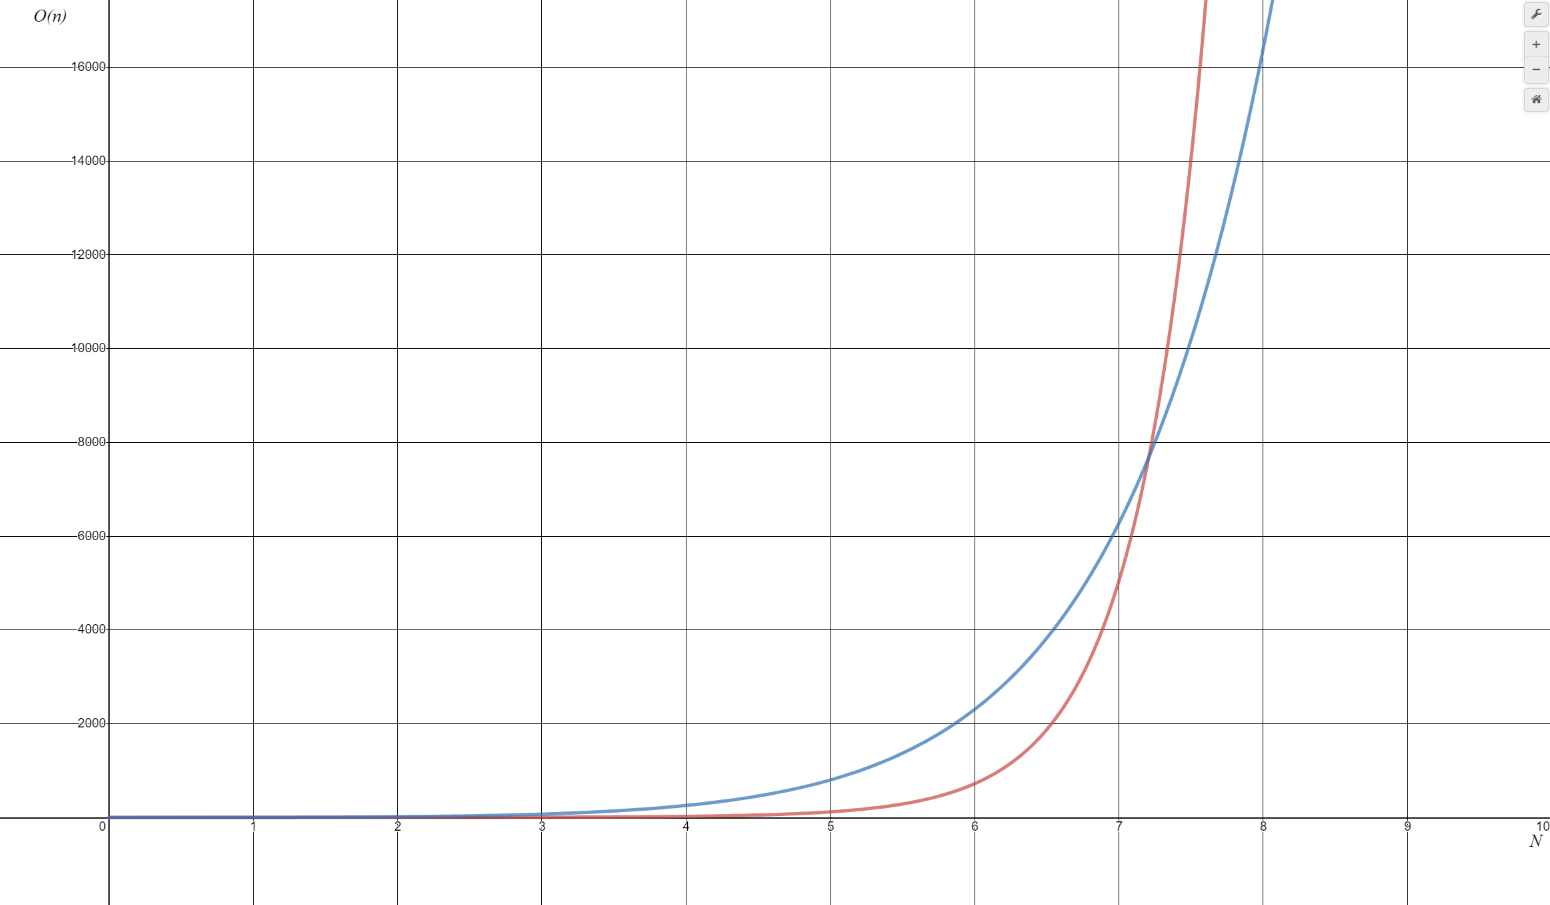
\includegraphics[scale=0.1]{tsp_exact_complexity}
\caption{\emph{Brute-force \textbf{vs.} Held-Karp algorithm: Complexities}}
\begin{tabular}{ l r }
\color{red} $-$ \color{black} Brute-force ($O(n!)$) & \color{blue} $-$ \color{black} Held-Karp ($O(n^22^n)$)
\end{tabular}
\end{figure}

Na implementação do cálculo da solução exata alternaríamos o método utilizado conforme o número de vértices a percorrer, usando brute-force para $n \leq 7$ e o algoritmo Held-Karp para $n > 7$.

\subsection{Soluções Aproximadas}
\subsubsection{Nearest Neighbour}
O algoritmo de \textbf{nearest neighbour} consiste em escolher um vértice aleatório para o início, e de seguida escolher o vértice mais próximo como próximo vértice a percorrer repetindo este passo até visitar todos os vértices a serem percorridos. Trata-se assim de algoritmo ganancioso que encontra uma solução aproximada em tempo reduzido, no entanto esta solução não é garantidamente a solução ótima.

O pseudo-código deste algoritmo é o seguinte:
\begin{lstlisting}[frame=single, mathescape=true]
FOR EACH v $\in$ V DO
  VISITED(v) $\leftarrow$ false
  PATH(v) $\leftarrow$ NULL

v $\leftarrow$ RANDOM_VERTEX(V) // choose starting point
VISITED(v) $\leftarrow$ true

WHILE NOT ALL_VISITED(V) DO
  w $\leftarrow$ CLOSEST_VERTEX(V, v) // get closest vertex to v
  VISITED(w) $\leftarrow$ v
  PATH(w) $\leftarrow$ v
  v $\leftarrow$ w
\end{lstlisting}

No nosso problema, o ponto inicial é fixo, sendo este a central, retirando assim a aleatoriedade do ponto inicial do algoritmo.

\subsubsection{Algoritmo Genético}
Algoritmos genéticos são algoritmos baseados em heurísticas que simulam o processo de evolução de espécies, a \href{https://en.wikipedia.org/wiki/Natural_selection}{\emph{seleção natural}}, selecionando os melhores espécimes de cada geração.

Os algoritmos genéticos podem ser divididos em cinco fases:
\begin{enumerate}
	\item Gerar a população
	\item Calcular a aptidão de cada indivíduo da população
	\item Escolher os indivíduos mais aptos
	\item Reproduzir os indivíduos escolhidos (por replicação ou \emph{crossover})
	\item Mutação dos indivíduos de modo a introduzir pequenas variações na população
\end{enumerate}

\begin{lstlisting}[frame=single, mathescape=true]
// calculate  fitness
CALCULATE_FITNESS(I)
  fitness $\leftarrow$ 0
  FOR i $\leftarrow$ 1 TO $\vert VERTICES(I) \vert$
    // add cost of going from vertex i-1 to vertex i
    fitness $\leftarrow$ fitness + COST(VERTICES[i-1], VERTICES[i])
  FITNESS(I) $\leftarrow$ fitness

// Choose the n best individuals
CULL_POPULATION(P, n)
  sorted $\leftarrow$ SORT_BY_FITNESS(P) // sort by descending order of fitness
  best $\leftarrow$ $\varnothing$
  FOR i $\leftarrow$ 0 TO n
    INSERT(best, sorted(i))
  RETURN best

// replicate individual
REPLICATE(I)
  return EXACT_COPY(I)

// create new individual from two parents
CROSSOVER(parent_A, parent_B)
  child $\leftarrow$ NEW_INDIVIDUAL()
  // being N the number of vertices to visit
  // random integer in [0, N[
  section_start $\leftarrow$ RANDOM_INT(0, N)
  // random integer in ]section_start, N[
  section_end $\leftarrow$ RANDOM_INT(section_start + 1, N)
  // copy random section from parent A
  FOR i $\leftarrow$ section_start TO section_end DO
    VERTICES(child) AT (i) $\leftarrow$ VERTICES(parent_A) AT (i)

  // fill remaining empty sections with genes from parent B
  FOR i $\leftarrow$ 0 TO N DO
    IF VERTICES(child) AT (i) = NULL
      VERTICES(child) AT (i) $\leftarrow$ VERTICES(parent_B) AT (i)
  RETURN CHILD

// mutate individual
MUTATE(I)
  v $\leftarrow$ RANDOM_VERTEX(VERTICES(I)) // choose random vertex
  w $\leftarrow$ RANDOM_VERTEX(VERTICES(I)) // choose another random vertex
  SWAP(v, w)

// using crossover to reproduce (can be done with replication)
// reproduces population P
REPRODUCE_POPULATION(P)
  NEW_P $\leftarrow$ $\varnothing$
  FOR i $\leftarrow$ 0 TO POPULATION_SIZE DO
    // choose parents (can be tested to be different parents)
    parent_A $\leftarrow$ RANDOM_INDIVIDUAL(P)
    parent_B $\leftarrow$ RANDOM_INDIVIDUAL(P)
    I $\leftarrow$ CROSSOVER(parent_A, parent_B)
    random $\leftarrow$ RANDOM_FLOAT(0, 1) // random number between 0 and 1
    IF random < MUTATION_RATE THEN
      MUTATE(I)
    INSERT(NEW_P, I)
  RETURN NEW_P


// generate random population (random order of vertices to visit)
P $\leftarrow$ GENERATE_RANDOM_POPULATION(V)

WHILE ... // decide stopping criteria
  FOR EACH individual $\in$ P
    CALCULATE_FITNESS(individual)

  best $\leftarrow$ CULL_POPULATION(P, n)
  P $\leftarrow$ REPRODUCE_POPULATION(best) // reproduce best individuals
\end{lstlisting}

De modo a garantir a restrição imposta sobre a ordem de visita dos locais de interesse, isto é, deve ser visitado o local de recolha antes do local de destino, podemos atribuir a aptidão mínima a todos os indíviduos que não respeitem tal restrição.

\newpage
%----------------------------------------------------------------------------------------
%	CHAPTER 4 - Funcionalidades a implementar
%----------------------------------------------------------------------------------------
\chapter[Funcionalidades a implementar][Funcionalidades a implementar]{Funcionalidades a implementar} \label{\thechapter}

\section{Pré-processamento dos dados de entrada}

\subsection{Grafo}
De modo a marcar todas as arestas alcançáveis a partir do vértice da central pode ser utilizada uma estratégia semelhante à procura em profundidade ($Depth-First Search$), começando a visita na central, e marcar todos os vértices que forem visitados como $open$.

O pseudo-código para esta estratégia é o seguinte:

\begin{lstlisting}[frame=single, mathescape=true]
VISIT(node)
  reachable(node) $\leftarrow$ true
  FOR w $\in$ Adj(node) DO
    IF NOT reachable(w) THEN
      VISIT(w)

// G - graph
// source - starting point
VISIT_FROM_SOURCE(G, source)
  FOR v $\in$ VERTICES(G) DO
    reachable(v) $\leftarrow$ false

  VISIT(source)
\end{lstlisting}

Para a identificação dos vértices do grafo que pertençam à componente fortemente conexa do vértice da central, será necessário analisar a conetividade do grafo e a construção do componente fortemente conexo, para o qual se destacam os algoritmos de Kosaraju e de Tarjan.

\subsubsection{Algoritmo de Kosaraju}

O algoritmo de Kosaraju consiste nos seguintes passos:
\begin{enumerate}
	\item Realizar uma pesquisa em profundidade no grafo colocando os vértices numa stack após visitar o vértice, obtendo assim os vértices em pós-ordem
	\item Transpor o grafo (inverter o sentido de todas as arestas)
	\item Fazer uma pesquisa em profundidade nos vértices pela ordem que estão definidos na stack. Depois de ser feita a pesquisa obtém-se a componente fortemente conexa a que esse vértice pertence
\end{enumerate}

No entanto, como no nosso caso só interessa saber a componente fortemente conexa relativa à central, podemos apenas percorrer o grafo transposto a partir desse mesmo vértice. \\

O pseudo-código para o algoritmo é, então, o seguinte:
\begin{lstlisting}[frame=single, mathescape=true]
// G - graph
// C - container to store the vertices of the SCC
DFS_VISIT(G, node, C)
  visited(node) $\leftarrow$ true
  FOR w $\in$ Adj(v) DO
    IF not visited(w) THEN
      DFS_VISIT(w)
  INSERT(C, node)

  GT $\leftarrow$ TRANSPOSE(G)

  SCC $\leftarrow$ $\varnothing$

  DFS_VISIT(GT, source, SCC)

\end{lstlisting}

A complexidade temporal de uma pesquisa em profundidade, assim como, a complexidade de inverter todas as arestas é proporcional ao tamanho do grafo isto é $O(|V| + |E|)$ sendo $|V|$ o número de vértices e $|E|$ o número de arestas.

Como o algoritmo de Kosaraju se baseia em duas pesquisas em profundidade e numa inversão do grafo realizadas sequencialmente a complexidade do algoritmo também é $O(|V| + |E|)$ (uma vez que a inserção, deleção e a obtenção do topo da stack são realizadas em tempo constante, $O(1)$, não afetando a complexidade temporal do algoritmo).

\subsection{Algoritmo de Tarjan}

O Tarjan é uma versão mais eficiente do algoritmo de Kosaraju, precisando apenas de realizar uma única pesquisa em profundidade para obter o grafo fortemente conexo.

Similarmente ao algoritmo de Kosaraju, o algoritmo de Tarjan também executa em tempo linear, $O(|V| + |E|)$, porém, este último baseia-se numa única pesquisa em profundidade, sendo assim mais eficiente.

Como no nosso caso apenas interessa saber a componente fortemente conexa a partir da central, este algoritmo não irá trazer muitas vantagens relativamente ao algoritmo visto anteriormente. Deste modo, a sua implementação não será uma prioridade, podendo ser considerada numa fase futura.

\newpage
\section{Casos de Implementação}
Perante a organização dos caminhos a percorrer pelos veículos, é necessário ter em consideração os seguintes aspetos:

\begin{itemize}
	\item Escolha do melhor percurso para um veículo
	\item Escolha dos pedidos de transporte de prisioneiros para cada veículo
	\item Agrupar os pedidos de prisioneiros
	\item Agrupar os veículos
\end{itemize}

Deve ter-se como objetivo a atribuição de uma carrinha a um serviço, tendo atenção aos prisioneiros que se precisam de transportar.

Devem ser, portanto, seguidos os seguintes passos quando é recebido um novo pedido de transporte de prisioneiros:

\begin{itemize}
	\item Ordenação dos serviços de modo a que os pedidos de transporte de prisioneiros mais antigos sejam analisados primeiro
	\item Escolha do veículo disponível que possa efetuar os pedidos que foram recebidos num determinado período de tempo
	\item Verificar se veículos que estão a executar algum pedido estão aptos à existência de novos pedidos de transporte de prisioneiros. Se um veículo puder efetuar esse pedido sem alterar o seu percurso, então o pedido deve ser sempre aceite
\end{itemize}

\newpage
\section{Casos de Utilização}

A aplicação a implementar irá incluir um menu de interação com o utilizador (GUI) capaz de navegar entre vários submenus, possibilitando o acesso às seguintes funcionalidades:

\begin{itemize}
	\item Visualização do grafo que contém o mapa disponibilizado (em GraphViewer)
	\item Cálculo otimizado do percurso entre dois pontos
	\item Adição e visualização do número de veículos
	\item Adição de novos pedidos
	\item Atribuição dos serviços tendo em conta os pedidos e as carrinhas disponíveis
\end{itemize}

Para adicionar novos pedidos, o utilizador terá que indicar o \textbf{local de recolha} e \textbf{destino dos prisioneiros}, o \textbf{número de prisioneiros}, \textbf{tipo de prisioneiros}, \textbf{peso da distância no trajeto} e o \textbf{peso do tempo no trajeto}.

Deste modo, a aplicação terá capacidade de gerir de uma forma otimizada e segura o transporte de passageiros entre diversos estabelecimentos, para além de armazenar a informação relativa aos percursos, permitindo a sua visualização.

\newpage
%----------------------------------------------------------------------------------------
%	CHAPTER 5 - Estruturas de dados utilizadas
%----------------------------------------------------------------------------------------
\chapter[Estruturas de dados utilizadas][Estruturas de dados utilizadas]{Estruturas de dados utilizadas} \label{\thechapter}

\section{Grafo}
O grafo que fora utilizado no desenvolvimento deste projeto é uma adaptação de um grafo fornecido previamente nesta mesma unidade curriculas, porém adaptado ao nosso problema. Para guardar os vértices e as 
arestas utilizamos um $vectors$ que contém um pointer para o respetivo elemento. Cada aresta e cada vértice possuem um ID que permitem a sua identificação.
Relativamente aos vértices, estes ainda possuem uma posição, as arestas que partem desse mesmo vértice, entre outros campos que são utilizados
na execução de diversos algoritmos.
Relativamente às arestas, estas possuem o vértice de destino e os peso do tempo e da distância. 
Estas classes referidas anteriormente encontram-se no diretório graph.

\section{Departamento}
O departamento possui o grafo, assim como um vetor que permite acessar todos os veículos disponíveis e todos os serviços a que este mesmo departamento tem de responder.
\subsection{Pedidos}
Cada pedido é caracterizado pelo número de prisioneiros e o tipo de transporte que vai ser necessário efetuar. Além disso, o pedido de transporte também possui o ponto 
em que vai ser efetuado o ponto de recolha e o ponto de destino, assim como o peso da distância e peso do tempo.

\subsection{Carrinhas}
Cada carrinha possui uma capacidade máxima, que corresponde ao número de prisioneiros que a mesma consegue transportar.

\subsection{Serviço}

\section{Algoritmos}
Ao longo das quatro iterações deste projeto utilizamos diversas estruturas de dados.

\subsection{Djisktra}
Para a implementação do algoritmo de Djisktra, utilizamos uma $MutablePriorityQueue$ já fornecida previamente. Esta possui a vantagem de ser possível alterar a \textit{key} 
de um elemento sem precisar de o remover e voltar a inserir na $PriorityQueue$.

\subsection{A-Star}
O algoritmo $A-Star$ é semelhante ao de Djisktra utilizando também uma $MutablePriorityQueue$. No entanto, além desta estrutura de dados, o algoritmo possui uma heurística que 
permite fazer uma estimativa do vértice que se poderá encontrar mais próximo do local de destino.

\subsection{Nearest Neighbour}
O algoritmo $Nearest Neighbour$ faz uso de $MultiMaps$ e $Sets$. Uma vez que é possível que vários pedidos tenham o mesmo ponto de recolha, a utilização de multimaps permite a
existência de Keys iguais, mas com pontos de destino diferentex.

\newpage
%----------------------------------------------------------------------------------------
%	CHAPTER 6 - Algoritmos efetivamente implementados e análise de complexidade 
%----------------------------------------------------------------------------------------
\chapter[Algoritmos efetivamente implementados][Algoritmos efetivamente implementados]{Algoritmos efetivamente implementados} \label{\thechapter}

Código para análise temporal empírica:

\section{Kosaraju}

\section{Pré processamento}

\section{Djisktra}
\subsection{Análise teórica}
\subsection{Análise temporal empírica}

\section{A-Star}
\subsection{Análise teórica}
\subsection{Análise temporal empírica}

\section{Nearest Neighbour}
\subsection{Análise teórica}
\subsection{Análise temporal empírica}

\newpage
%----------------------------------------------------------------------------------------
%	CHAPTER 7 - Conectividade dos grafos utilizados
%----------------------------------------------------------------------------------------
\chapter[Conectividade dos grafos utilizados][Conectividade dos grafos utilizados]{Conectividade dos grafos utilizados} \label{\thechapter}

Conforme foi referido anteriormente, antes de começar a procura do caminho mais curto é necessário verificar que todos os pontos de interesse a serem percorridos encontram-se na
parte fortemente conexa do grafo. Para garantir isto foi utilizado o algoritmo de $Kosaraju$ que permite obter a parte fortemente conexa do grafo. Depois deste algoritmo ser aplicado
é possível distinguir através do $GraphViewer$ as componentes do grafo que se encontram conexas dos componentes que não se encontram conexos atráves da sua cor. Os vértices e arestas
que se encontram representados com a cor vermelha, correspondem àqueles que se encontram na parte não conexa do grafo. Respetivamente, aqueles elementos que se encontram com cor
verde correspondem à parte conexa do grafo.

\section{Grafos pouco conexos}
Foi utilizado um grafo pouco conexo para verificar que o nosso algoritmo de $Kosaraju$ estava bem implementado. O mapa pouco conexo utilizado foi do $Porto$.

\section{Grafos muito conexos}
Os grafos conexos foram utilizados para testar as diversas iterações, uma vez que estes permitem visitar quase todos os vértices. Foram utilizados os $GridMaps$ $8x8$ e $16x16$,
assim como o mapa de $Cabeceiras$.

\newpage
%----------------------------------------------------------------------------------------
%	CHAPTER 8 - Conclusão
%----------------------------------------------------------------------------------------
\chapter[Conclusão][Conclusão]{Conclusão} \label{\thechapter}

O objetivo deste trabalho foi o desenvolvimento de uma estratégia responsável pela atribuição de veículos e rotas, através da criação de um modelo capaz de otimizar a resolução deste problema.

O modelo foi dividido em três iterações, sendo as primeiras duas problemas do tipo \textbf{caminho mais curto entre dois vértices}. A terceira e a última iteração são equiparadas aos problemas: \textbf{Travelling Salesman Problem} e \textbf{Vehicle Routing Problem}.

Foram utilizados múltiplos algoritmos no sentido de resolver estes problemas, nomeadamente \textbf{Dijkstra}, \textbf{A*}, \textbf{Held-Karp}, \textbf{Nearest Neighbour},\textbf{Genético}, \textbf{Kosaraju} e \textbf{Tarjan}.

Estes algoritmos envolvem conhecimentos em várias áreas da programação, transpondo os conceitos abordados na cadeira, tais como: \textbf{bruteforce}, \textbf{recursão}, \textbf{programação dinâmica}, \textbf{algoritmos gananciosos} (\textbf{Dijkstra}, \textbf{A*}, \textbf{Nearest Neighbour}), \textbf{heurísticas}, vários conceitos associados a algoritmos genéticos, tais como, \textbf{mutação}, \textbf{crossover}, \textbf{seleção} e outros tópicos associados a grafos, nomeadamente, \textbf{conetividade} e  \textbf{ordem topológica}.

Cada membro do grupo foi responsável por uma igual parte do trabalho, sendo cada um responsável pelas seguintes partes do projeto:
\begin{itemize}
	\item\emph{ Diogo Samuel Fernandes} - Descrição do Problema, Perspetiva de solução, Pré-processamento dos dados de entrada (Funcionalidades a implementar),  Conclusão
	\item\emph{ Hugo Guimarães} -  Perspetiva de solução, Funcionalidades a implementar, Conclusão
	\item\emph{ Telmo Baptista} - Formalização do Problema, Perspetiva de solução, Pré-processamento dos dados de entrada (Funcionalidades a implementar),  Conclusão
\end{itemize}

\newpage
\chapter{Bibliografia}
\begin{itemize}
	\item Apresentações fornecidas pelo professor Rosaldo José Fernandes Rossetti nas aulas téoricas da cadeira \href{https://sigarra.up.pt/feup/pt/ucurr_geral.ficha_uc_view?pv_ocorrencia_id=436441}{Conceção e Análise de Algoritmos}
	\item Shortest Path Problem,\\
	\color{blue} \underline{\href{https://en.wikipedia.org/wiki/Shortest_path_problem}{https://en.wikipedia.org/wiki/Shortest\_path\_problem}} \color{black}
	\item Dijkstra's Algorithm,\\
	\color{blue} \underline{\href{https://en.wikipedia.org/wiki/Dijkstra\%27s_algorithm}{https://en.wikipedia.org/wiki/Dijkstra\%27s\_algorithm}} \color{black}
	\item Bellman-Ford Algorithm,\\
	\color{blue} \underline{\href{https://en.wikipedia.org/wiki/Bellman\%E2\%80\%93Ford_algorithm}{https://en.wikipedia.org/wiki/Bellman\%E2\%80\%93Ford\_algorithm}} \color{black}
	\item A* algorithm,\\
	\color{blue} \underline{\href{https://en.wikipedia.org/wiki/A*_search_algorithm}{https://en.wikipedia.org/wiki/A*\_search\_algorithm}} \color{black}
	\item Admissible heuristic,\\
	\color{blue} \underline{\href{https://en.wikipedia.org/wiki/Admissible_heuristic}{https://en.wikipedia.org/wiki/Admissible\_heuristic}} \color{black}
	\item Traveling Salesman Problem,\\
	\color{blue} \underline{\href{https://en.wikipedia.org/wiki/Travelling_salesman_problem}{https://en.wikipedia.org/wiki/Travelling\_salesman\_problem}} \color{black}
	\item Vehicle Routing Problem,\\
	\color{blue} \underline{\href{https://en.wikipedia.org/wiki/Vehicle_routing_problem}{https://en.wikipedia.org/wiki/Vehicle\_routing\_problem}} \color{black}
	\item Held-Karp algorithm,\\
	\color{blue} \underline{\href{https://en.wikipedia.org/wiki/Held\%E2\%80\%93Karp_algorithm}{https://en.wikipedia.org/wiki/Held\%E2\%80\%93Karp\_algorithm}} \color{black}
	\item Nearest neighbour algorithm,\\
	\color{blue} \underline{\href{https://en.wikipedia.org/wiki/Nearest_neighbour_algorithm}{https://en.wikipedia.org/wiki/Nearest\_neighbour\_algorithm}} \color{black}
	\item Genetic Algorithm,\\
	\color{blue} \underline{\href{https://en.wikipedia.org/wiki/Genetic_algorithm}{https://en.wikipedia.org/wiki/Genetic\_algorithm}} \color{black}
	\item Natural selection,\\
	\color{blue} \underline{\href{https://en.wikipedia.org/wiki/Natural_selection}{https://en.wikipedia.org/wiki/Natural\_selection}} \color{black}
	\item DNA replication,\\
	\color{blue} \underline{\href{https://en.wikipedia.org/wiki/DNA_replication}{https://en.wikipedia.org/wiki/DNA\_replication}} \color{black}
	\item Chromosomal crossover,\\
	\color{blue} \underline{\href{https://en.wikipedia.org/wiki/Chromosomal_crossover}{https://en.wikipedia.org/wiki/Chromosomal\_crossover}} \color{black}
	\item Mutation,\\
	\color{blue} \underline{\href{https://en.wikipedia.org/wiki/Mutation}{https://en.wikipedia.org/wiki/Mutation}} \color{black}
	\item GeeksForGeeks - Strongly connected components,\\
	\color{blue} \underline{\href{https://www.geeksforgeeks.org/strongly-connected-components}{https://www.geeksforgeeks.org/strongly-connected-components}} \color{black}
	\item Kosaraju's algorithm,\\
	\color{blue} \underline{\href{https://en.wikipedia.org/wiki/Kosaraju\%27s_algorithm}{https://en.wikipedia.org/wiki/Kosaraju\%27s\_algorithm}} \color{black}
	\item Tarjan's algorithm,\\
	\color{blue} \underline{\href{https://en.wikipedia.org/wiki/Tarjan\%27s_strongly_connected_components_algorithm}{https://en.wikipedia.org/wiki/Tarjan\%27s\_strongly\_connected\_components\_algorithm}} \color{black}
	\item GeeksForGeeks - Tarjan's algorithm,\\
	\color{blue} \underline{\href{https://www.geeksforgeeks.org/tarjan-algorithm-find-strongly-connected-components}{https://www.geeksforgeeks.org/tarjan-algorithm-find-strongly-connected-components}} \color{black}
	\item Desmos Graphing Tool,\\
	\color{blue} \underline{\href{https://www.desmos.com/calculator}{https://www.desmos.com/calculator}} \color{black}
	\item Path Finder Visualization Program,\\
	\color{blue} \underline{\href{https://github.com/kevinwang1975/PathFinder}{https://github.com/kevinwang1975/PathFinder}} \color{black}
	\item Branch and Bound,\\
	\color{blue} \underline{\href{https://en.wikipedia.org/wiki/Branch_and_bound}{https://en.wikipedia.org/wiki/Branch\_and\_bound}} \color{black}
\end{itemize}

\end{document}

\end{document}
